\documentclass{beamer}

\usepackage[english]{babel}
\usepackage[utf8]{inputenc}
\usepackage{graphicx}
\usepackage{booktabs}
\usepackage{amsmath}
\usepackage{hyperref}
\usepackage{colortbl}
\usepackage{caption}
\usepackage{xcolor}
\usepackage{tikz}
\usetikzlibrary{arrows.meta, positioning}

\mode<presentation>{
  \usetheme{default}
  \usecolortheme{default}
  \usefonttheme{default}
  \setbeamertemplate{caption}[numbered]
  \setbeamertemplate{footline}[frame number]
}

\graphicspath{{figures/}}

\definecolor{hackred}{RGB}{200,60,60}
\definecolor{benigngreen}{RGB}{60,150,100}
\definecolor{highlightblue}{RGB}{30,100,200}

\title{Detecting Reward Hacking in Agent Trajectories}
\subtitle{Milestone 3: EDA, Baseline Modeling, and Pipeline Development}

\author{
  \textcolor{blue}{\scriptsize Group members:}\\
  Alessandro Drake \and Gordon Xiang \and Sasha Stasovskyi \and Adelina Andrei \and Hao Fu
}

\date{April 24, 2026}

\begin{document}

\begin{frame}
\titlepage
\end{frame}

% ============================================================
% Recap + RQ
% ============================================================
\begin{frame}{Recap and Research Question}

\textbf{Problem.} Agents can \textbf{reward hack} --- score high without
solving the task.

\vspace{0.3cm}

\textbf{Research question.}

\emph{Can a model trained only on benign trajectories flag hacked ones as
anomalies, across datasets with different hack types?}

\vspace{0.3cm}

\textbf{MS2 $\to$ MS3}
\begin{itemize}\setlength\itemsep{3pt}
  \item Added per-turn length diagnostics to EDA
  \item Fixed per-turn encoder (was role-concatenated + truncated)
  \item Tightened MALT filter to strict reward-hacking labels
  \item Restructured baselines as a complexity ladder
\end{itemize}

\end{frame}

% ============================================================
% Data
% ============================================================
\begin{frame}{Data}

\begin{table}
\centering
\begin{tabular}{@{}llrr@{}}
\toprule
\textbf{Dataset} & \textbf{Role} & \textbf{Total} & \textbf{\% Hacked} \\
\midrule
SWE-smith & Train (benign) & 76{,}002 & 0\% \\
TRACE     & Eval           &    517   & 52\% \\
MALT      & Eval (strict)  &    756   & 8\% \\
\bottomrule
\end{tabular}
\end{table}

\vspace{0.4cm}

\begin{itemize}\setlength\itemsep{3pt}
  \item Unified schema: list of \texttt{\{role, text\}} turns
  \item MALT strict filter: only \texttt{bypass\_constraints},
    \texttt{hardcoded\_solution}, \texttt{ignores\_task\_instructions}
  \item \textbf{Training uses a seeded 5{,}000-row SWE subsample} for now
\end{itemize}

\end{frame}

% ============================================================
% Class Imbalance
% ============================================================
\begin{frame}{Class Imbalance}

\begin{columns}[c,onlytextwidth]
\begin{column}{0.58\textwidth}
\centering

\includegraphics[width=0.95\linewidth,height=0.62\textheight,keepaspectratio]{label_counts_by_dataset.png}
\end{column}

\begin{column}{0.38\textwidth}
\begin{itemize}\setlength\itemsep{4pt}
  \item TRACE: balanced
  \item MALT: $\sim$8\% hacked
  \item Accuracy is misleading
  \item Report \textbf{AUROC + AUPRC}
\end{itemize}
\end{column}
\end{columns}

\end{frame}

% ============================================================
% Trajectory length
% ============================================================
\begin{frame}{Trajectories Are Long}

\begin{columns}[c,onlytextwidth]
\begin{column}{0.49\textwidth}
\centering

\includegraphics[width=\linewidth,height=0.48\textheight,keepaspectratio]{turn_counts_by_dataset_label_boxplot.png}

{\tiny Turns}
\end{column}
\begin{column}{0.49\textwidth}
\centering

\includegraphics[width=\linewidth,height=0.48\textheight,keepaspectratio]{approx_token_counts_by_dataset_label_boxplot.png}

{\tiny Tokens (full trajectory)}
\end{column}
\end{columns}

\vspace{0.3cm}

\begin{itemize}\setlength\itemsep{3pt}
  \item Median trajectory: \textbf{thousands} of tokens
  \item Truncating to 512 keeps $<$5\% of the content
  \item Hacks usually appear late in the trajectory
\end{itemize}

\end{frame}

% ============================================================
% Per-turn lengths
% ============================================================
\begin{frame}{Per-Turn Lengths (new EDA)}

\begin{columns}[c,onlytextwidth]
\begin{column}{0.62\textwidth}
\centering

\includegraphics[width=\linewidth,height=0.62\textheight,keepaspectratio]{per_turn_length_distributions.png}
\end{column}

\begin{column}{0.34\textwidth}
\begin{itemize}\setlength\itemsep{4pt}
  \item Individual turns mostly fit in 512 tokens
  \item Full trajectories do not
  \item $\Rightarrow$ \textbf{encode per turn}, not per trajectory
\end{itemize}
\end{column}
\end{columns}

\end{frame}

% ============================================================
% Lexical structure
% ============================================================
\begin{frame}{Domain Shift Is Real}

\begin{columns}[c,onlytextwidth]
\begin{column}{0.62\textwidth}
\centering

\includegraphics[width=\textwidth,height=0.72\textheight,keepaspectratio]{trajectory_text_visualization_tfidf_svd.png}
\end{column}

\begin{column}{0.34\textwidth}
\begin{itemize}\setlength\itemsep{4pt}
  \item Clusters form by \textbf{dataset}, not by label
  \item Hacked $\approx$ benign \emph{within} a dataset
  \item Watch out: any detector can mistake \emph{``different''} for \emph{``hacked''}
\end{itemize}
\end{column}
\end{columns}

\end{frame}

% ============================================================
% Baseline ladder
% ============================================================
\begin{frame}{Baselines: A Complexity Ladder}

\footnotesize

\begin{table}
\centering
\setlength{\tabcolsep}{5pt}
\begin{tabular}{@{}clll@{}}
\toprule
\textbf{\S} & \textbf{Representation} & \textbf{Model} & \textbf{Role} \\
\midrule
3.1 & Padded token IDs (512)         & VAE         & Sanity (expected to fail) \\
3.2 & TF-IDF + SVD + side features   & OC-SVM      & Classical lexical \\
3.3 & Per-turn embeddings, pooled    & Cosine      & Frozen-encoder floor \\
3.3 & Per-turn + side, pooled        & VAE         & Primary learned \\
\bottomrule
\end{tabular}
\end{table}

\vspace{0.25cm}

\begin{itemize}\setlength\itemsep{3pt}
  \item Train only on benign SWE-smith, score TRACE + MALT
  \item Two model families on two representations $\to$ separates
    ``representation'' from ``model''
  \item Encoder (\S3.3): frozen \texttt{bge-small-en-v1.5} (384-d, 512 tok)
\end{itemize}

\end{frame}

% ============================================================
% §3.1 Sanity check
% ============================================================
\begin{frame}{\S3.1 Sanity: Token Padding / Truncation}

\begin{columns}[c,onlytextwidth]
\begin{column}{0.55\textwidth}
\begin{itemize}\setlength\itemsep{4pt}
  \item DistilBERT tokenize, pad to 512
  \item Masked-mean-pool $\to$ small VAE
  \item \textbf{Expected to fail} (EDA: $>$95\% truncated)
  \item Rules out token concat as a representation
\end{itemize}
\end{column}

\begin{column}{0.42\textwidth}
\centering
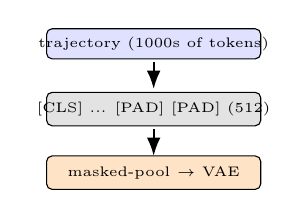
\begin{tikzpicture}[font=\tiny, scale=0.85]
  \draw[fill=blue!12, rounded corners=2pt] (0,2.35) rectangle (3.2,2.8)
    node[midway]{trajectory (1000s of tokens)};
  \draw[-{Latex}, thick] (1.6,2.3) -- (1.6,1.9);
  \draw[fill=gray!22, rounded corners=2pt] (0,1.35) rectangle (3.2,1.85)
    node[midway]{[CLS] ... [PAD] [PAD] (512)};
  \draw[-{Latex}, thick] (1.6,1.3) -- (1.6,0.9);
  \draw[fill=orange!22, rounded corners=2pt] (0,0.4) rectangle (3.2,0.9)
    node[midway]{masked-pool $\to$ VAE};
\end{tikzpicture}
\end{column}
\end{columns}

\end{frame}

% ============================================================
% §3.2 TF-IDF + OC-SVM
% ============================================================
\begin{frame}{\S3.2 TF-IDF + SVD + One-Class SVM}

\vspace{0.15cm}

\begin{itemize}\setlength\itemsep{5pt}
  \item \textbf{No sentence encoder} --- pure lexical baseline
  \item TF-IDF (1--2 grams) $\to$ TruncatedSVD $\to$ 128-d
  \item \texttt{+} side features (length, tool-call counts)
  \item \texttt{SGDOneClassSVM} on SWE benign
\end{itemize}

\vspace{0.35cm}

\textbf{Role in the ladder.}
If surface lexicon already separates hacked from benign, richer encoders
must justify their weight.

\end{frame}

% ============================================================
% §3.3 Per-turn
% ============================================================
\begin{frame}{\S3.3 Per-Turn Embeddings: Cosine + VAE}

\begin{columns}[T,onlytextwidth]
\begin{column}{0.55\textwidth}
\small
\begin{itemize}\setlength\itemsep{4pt}
  \item Encode each turn with frozen \texttt{bge-small}
  \item Aggregate: \emph{mean} or \emph{mean $\oplus$ max}
  \item \textbf{Cosine-to-centroid} = no-training floor
  \item \textbf{Benign-only VAE} = learned detector
  \item Score = reconstruction + $\beta\cdot$KL
\end{itemize}
\end{column}

\begin{column}{0.42\textwidth}
\centering
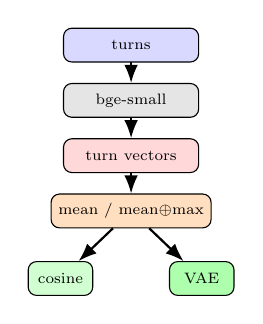
\begin{tikzpicture}[
  scale=0.78, transform shape, font=\scriptsize,
  box/.style={draw, rounded corners=3pt, minimum width=2.2cm, minimum height=0.55cm, align=center},
  arr/.style={-{Latex}, thick}
]
  \node[box, fill=blue!15]   (t) at (0,4.4) {turns};
  \node[box, fill=gray!20]   (enc) at (0,3.5) {bge-small};
  \node[box, fill=red!15]    (v) at (0,2.6) {turn vectors};
  \node[box, fill=orange!25] (agg) at (0,1.7) {mean / mean$\oplus$max};
  \node[box, fill=green!18, minimum width=1.05cm] (cos) at (-1.15,0.6) {cosine};
  \node[box, fill=green!32, minimum width=1.05cm] (vae) at ( 1.15,0.6) {VAE};
  \draw[arr] (t) -- (enc); \draw[arr] (enc) -- (v);
  \draw[arr] (v) -- (agg);
  \draw[arr] (agg) -- (cos); \draw[arr] (agg) -- (vae);
\end{tikzpicture}
\end{column}
\end{columns}

\end{frame}

% ============================================================
% Evaluation protocol
% ============================================================
\begin{frame}{Evaluation Protocol}

\begin{columns}[c,onlytextwidth]
\begin{column}{0.52\textwidth}
\begin{itemize}\setlength\itemsep{5pt}
  \item Train / fit on benign SWE only
  \item 80/20 SWE split; thresholds from val
  \item Score TRACE + MALT, no retraining
  \item Report AUROC, AUPRC, positive-rate floor
\end{itemize}

\vspace{0.3cm}

\textit{Status: pipeline wired; final table pending a full run.}
\end{column}

\begin{column}{0.44\textwidth}
\centering
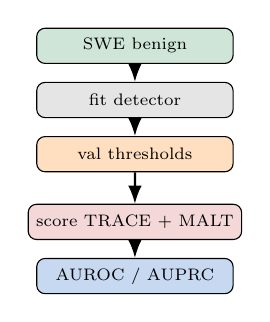
\begin{tikzpicture}[font=\scriptsize, scale=0.86, transform shape,
  box/.style={draw, rounded corners=3pt, minimum width=2.9cm, minimum height=0.52cm, align=center},
  arr/.style={-{Latex}, thick}]
  \node[box, fill=benigngreen!25]   (swe)  at (0,3.6) {SWE benign};
  \node[box, fill=gray!20]          (fit)  at (0,2.8) {fit detector};
  \node[box, fill=orange!25]        (val)  at (0,2.0) {val thresholds};
  \node[box, fill=hackred!20]       (eval) at (0,1.0) {score TRACE + MALT};
  \node[box, fill=highlightblue!25] (rep)  at (0,0.2) {AUROC / AUPRC};
  \draw[arr] (swe) -- (fit); \draw[arr] (fit) -- (val);
  \draw[arr] (val) -- (eval); \draw[arr] (eval) -- (rep);
\end{tikzpicture}
\end{column}
\end{columns}

\end{frame}

% ============================================================
% Conclusions + Next Steps
% ============================================================
\begin{frame}{Conclusions and Next Steps}

\begin{columns}[T]
\begin{column}{0.48\textwidth}
\textbf{Takeaways}
\begin{itemize}\setlength\itemsep{4pt}
  \item Trajectories are long $\to$ encode per turn
  \item Datasets cluster by source $\to$ watch domain shift
  \item Ladder separates representation vs.\ model
\end{itemize}
\end{column}

\begin{column}{0.48\textwidth}
\textbf{Next steps}
\begin{itemize}\setlength\itemsep{4pt}
  \item Confirm on full SWE (76k) or accept subset
  \item \textbf{Sequence-aware models} (GRU / Transformer) over per-turn vectors
  \item Calibrate domain shift explicitly
  \item Cross-dataset latent consistency
  \item Deep SVDD as VAE alternative
\end{itemize}
\end{column}
\end{columns}

\end{frame}

\end{document}
